\documentclass[11pt]{article}

\usepackage{sectsty}
\usepackage{graphicx}
\usepackage{hyperref}

\graphicspath{./images/}

\topmargin=-0.45in
\evensidemargin=0in
\oddsidemargin=0in
\textwidth=6.5in
\textheight=9.0in
\headsep=0.25in

\title{Modifications to Linux Kernel Networking Stack}
\author{Nicholas Orlowsky}
\date{\today}

\begin{document}
\maketitle	


\section{Background}

Generally, NICs operate with a Maximum Transmission Unit (MTU) of 1500. This means that the maximum Ethernet 
frame size that they will support will be 1500 bytes. When dealing with a high volume of network traffic, it 
is common to increase the MTU to use `jumbo frames.' Doing so has advantages in certain use cases (such as large file transfers) where you're 
able to send data in large chunks, avoiding the overhead of processing more packets. However, some use cases cannot benefit from larger MTU 
sizes. One specific example is low-latency financial applications. The message sizes on a data feed from 
NYSE range from 20 to 76 bytes, far lower than the default MTU size on most NICs\cite{nyse}. These messages can't 
be batched into one larger message, as doing so would intrinsically introduce latency which is critical for 
consumers of this data feed.

The Linux Kernel isn't built to efficiently handle large amounts of small ethernet frame sizes. This makes processing 
these messages in an efficient manner time consuming. Alternative network stacks such as DPDK allow more 
customization, however, they're also generally built for general overall performance, not targeted performance 
in the use case of very small MTUs. Alternative network stacks also complicate deployment, as you become restricted 
in the NICs you can use and you must port your application to the stack. Making improvements to the kernel 
can provide both easier deployment, development, and better performance. 

This project aims to make significant gains in the time it takes for the recvmmsg() system call to return a set of 
UDP messages by modifying the Linux kernel.

The general case being optimized for is the pseudocode below. This test lets us measure how fast we can rx packets without any 
processing (besides basic validation), representing the fastest speed that data could be read.

\begin{verbatim}
    while(true) {
        struct mmsghdr headers[10000];
        recvmmsg(&headers);

        for(message in headers) {
            check_contents(message);
        }
    }
\end{verbatim}


\section{Design}

This section will detail the design decisions made when making modifications to the kernel to improve speed.

\subsection{Branching Behavior}

The likely() and unlikely() macros in the kernel to optimize branching decisons. They do this by giving the compiler 
hints about the outcome of a branghing result so that the compiler can favor that branching result when generating 
assembly. For example in the below code, we know that users will likely enter an even number most of the time, therefore 
we can wrap the conditional in a likely() macro so that the compiler generates code that favors the first branch:

\begin{verbatim}
    #include <stdio.h>

    int main() {
        while(1 == 1) {
            printf("Enter an even number: ");
            int num;
            scanf("%d", &num);
    
            if (likely(num % 2 == 0)) {
                printf("%d is a cool number!\n");
            } else {
                printf("That's an odd number. Please enter an even number.\n");
            }
        }
    }
\end{verbatim}

The generated assemply for variations of this with likely() and unlikely() are shown below (gcc x86\_64 14.2):


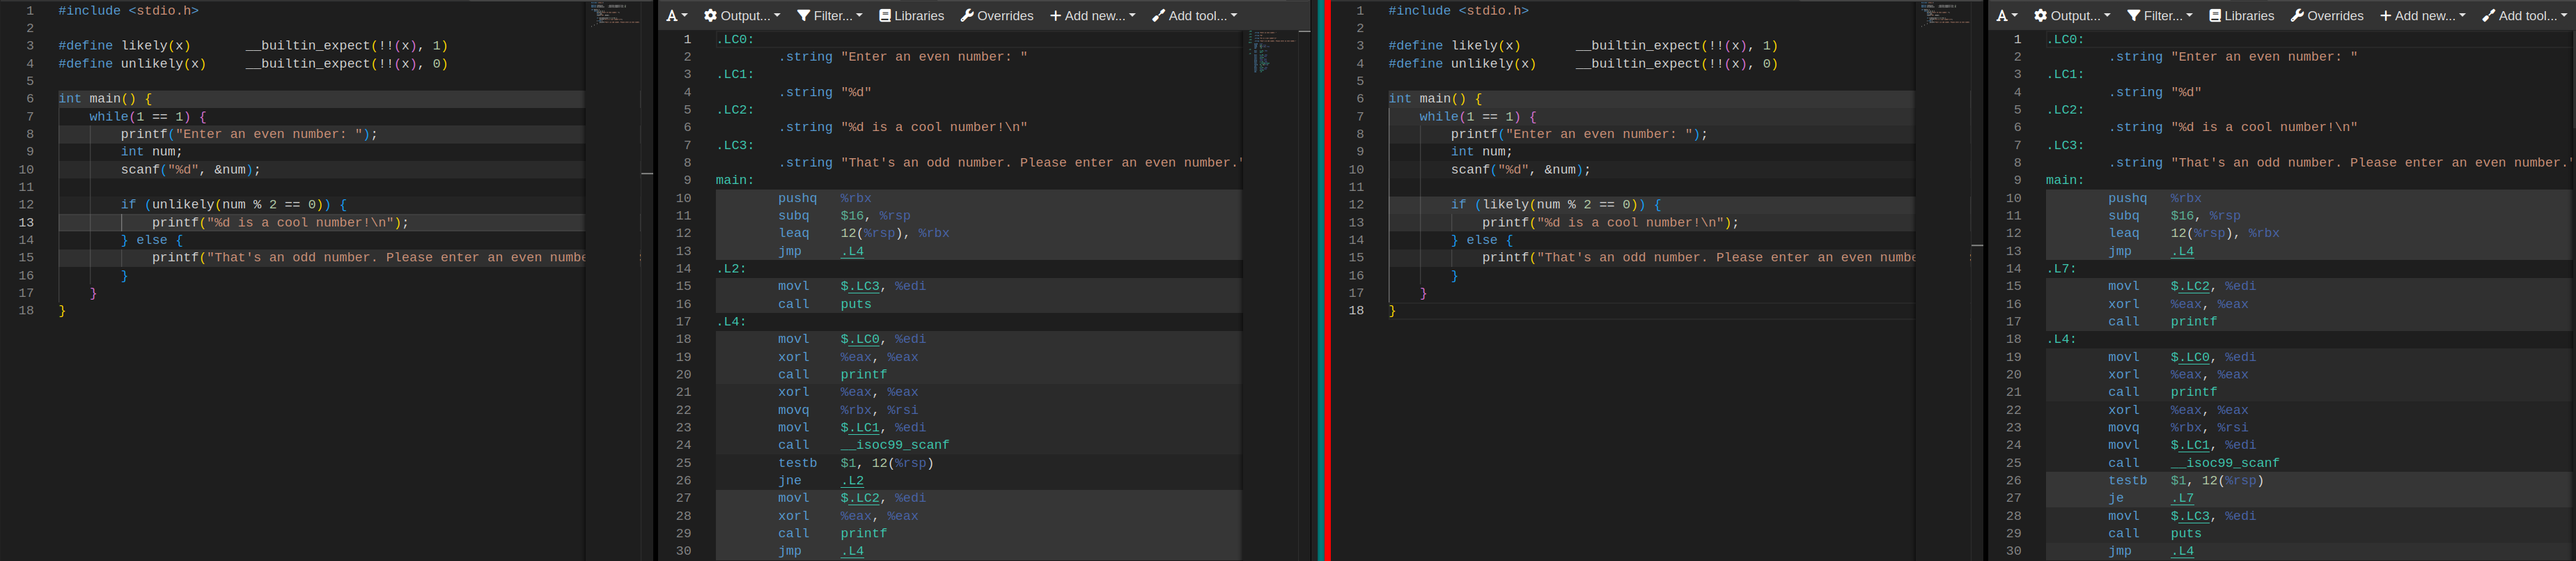
\includegraphics[width=17cm]{./images/godbolt.png}

The main difference is that line 26/27 where the jump from the if statement is has been flipped from a jne to a je, and that 
the contents of .L2/.L7 are both different ends of the if statement. 

The codepath down the kernel for the usecase mentioned in the Background section was annotated with these macros where appropriate 
to make the path that our code takes the preferred one by branch predictors.

The performance gains from this on modern microarchitectures are extrememly minor as modern branch predictors are very mature 
and good at predicting. If the tests were run on an old x86 processor or an older architecture such as MIPS, this may have 
yielded larger performance benefits.


\subsection{remember\_mmsghdr System Call}

The recvmmsg system call is a system call that recieves multiple messages from a socket. Under the lood, it calls recvmsg, a system 
call that recieves a single message from a socket multiple times. 

One of the parameters passed to recvmmsg is an array of mmsghdr structs. Within the mmsghdr struct, it contains a msghdr. The msghdr 
struct contains some control information and a buffer to copy message data into. 

When recvmmsg is called, the mmsghdr array is copied into the kernel. This copy happens on every invocation of recvmmsghdr. 
However, between invocations of the function, the contents of mmsghdr don't change in a meaningful way. This means that every iteration 
of the loop shown in previous sections that we're unnecessairly doing a large copy. For an array of 1000 128 byte messages, the total 
to copy is 208 Kb. 

To fix this behavior, I created the remember\_mmsghdr() system call. This sytem call takes in the mmsghdr array as a parameter and copies 
it into the kernel. When calling recvmmsg() afterwards, it will use the copy already present in the kernel instead of copying it in 
again, reducing the number of copies. An example invocation of the system call is below:

\begin{verbatim}
    remember_mmsghdr(listen_sock, &msgs[0], BUF_LEN, 0);
\end{verbatim}

This was implemented by adding a new struct to the kernel called mmsghdr\_state:

\begin{verbatim}
    struct mmsghdr_state {
        short present;               // Is cached mmsghdr state present in kernel 
        struct mmsghdr* address;     // Array of mmsghdr structs
        struct sockaddr** uaddrs;    // Array of sockaddr pointers
        struct iovec** iovecs;       // Array of iovec pointers
        unsigned int vlen;           // Number of mmsghdr structs
    };
\end{verbatim}

\textbf{struct socket} was then updated to contain an instance of mmsghdr\_state. Whenever remember\_mmsghdr() is called, the memory for 
the data is allocated in the kernel, and then recvmsg\_copy\_msghdr() is called to copy the msghdrs in the mmsghdr array into the kernel 
buffers. This is the same kernel function used by recvmsg and recvmmsg to copy the data into the kernel. After this completes, the vlen 
and present attributes of mmsghdr\_state are updated. Repeated attempts to call remember\_mmsghdr fail. This is discussed further in 
the Limitations section. 

On all subsequent calls to recvmmsg, the \textbf{struct mmsghdr\_state}'s present property is checked. If it isn't set, it runs the 
regular code to handle the copy. If it is set, then it skips the copy function and uses the pointers present in \textbf{struct mmsghdr\_state}.

Care needs to be taken to change the metadata of the \textbf{msg\_iter} property of the \textbf{struct msghdr} present in the kernel. There is 
some book-keeping data that marks how much data was written to the buffers storing the message data. If this isn't reset, the first call to 
recvmmsg() will behave normally, but subsequent calls will return the same data as the first call.

\subsubsection{Limitations \& Hacks}

There are a number of limitations and/or hacks that would cause Linus to have a meltdown and reject these patches that are present in this implementation
due to time constraints. 

As previously mentioned, subsequent calls to remember\_mmsghdr fail. Ideally, the behavior for this would be to update the contents of 
\textbf{struct mmsghdr\_state} in the kernel with the new data. This was left out due to not being a usecase covered in our tests and time constraints.

When using remember\_mmsghdr(), the system cal recvmsg (that's with one m, not 2) breaks. This is because in the kernel, recvmmsg just calls 
recvmsg in a loop, and the logic for using the in-kernel copies of mmsghdr are implemented in the recvmsg system call. There is likely a hacky 
way to make it work, but as of now it is undefined behavior and not implemented. This was left out due to not being a usecase covered in our tests and time constraints.

This implementation does not support the multithreaded use of remember\_mmsghdr with the same socket. Typically, after creating a socket, you may 
spawn multiple threads that call recvmmsg in a loop, much like the example in the introduction of this paper. When you do this, typically each thread has 
its own \textbf{struct mmsghdr*} array that it passes to recvmmsg(). Since the implementation only keeps one copy fo the mmsghdr state in the 
kernel per socket, this makes it ineffective to use across multiple threads. Additionally, access to \textbf{struct msmghdr\_state} isn't synchronized 
which could cause a slew of issues if used in a multithreaddes context. In the future to support this, the remember\_mmsghdr() state could 
include a table with the userspace address of the mmsghdr array mapped to it's kernel counterpart. This would allow the kernel to keep track of 
multiple copies of a mmsghdr array for one kernel. Of course, this would also require adding synchronization to manage this table. 

\section{Results}

\subsection{Local Experiment}

The local experiment measures the time it takes to transmit 100 million packets from 2 programs running on the same host machine in a VM. This test 
gives insight into a 'perfect-world' where the main bottlenecks will be the kernel code itself. This allows us to isolate the overhead gained with 
these patches without noise from interacting with another device on the network or with the NIC.

The test setup is the below:

\begin{itemize}
    \item \textbf{Machine CPU:} Ryzen 5 1600U 6 cores, 12 threads @ 3.2 GHz
    \item \textbf{Machine RAM:} 16 GB DDR4
    \item \textbf{Host Machine Kernel:} Linux 6.11.8-zen1-2-zen 
    \item \textbf{Guest Machine CPU:} 8 cores, 8 threads
    \item \textbf{Guest Machine RAM:} 8GB 
    \item \textbf{Guest Machine Kernel (modified):} Linux 6.11.0-rc6-aos-flab (custom built kernel)
    \item \textbf{Guest Machine Kernel (stock):} Linux 6.11.0-rc6-aos-flab (custom built kernel)
\end{itemize}

%\begin{itemize}
%    \item \textbf{Host Machine CPU:} Ryzen 5 1600U 6 cores, 12 threads @ 3.2 GHz
%    \item \textbf{Host Machine RAM:} 16 GB DDR4
%    \item \textbf{Host Machine Kernel:} Linux 6.11.8-zen1-2-zen 
%    \item \textbf{Guest Machine CPU:} 8 cores, 8 threads
%    \item \textbf{Guest Machine RAM:} 8GB 
%    \item \textbf{Guest Machine Kernel (modified):} Linux 6.11.0-rc6-aos-flab (custom built kernel)
%    \item \textbf{Guest Machine Kernel (stock):} Linux 6.11.0-rc6-aos-flab (custom built kernel)
%\end{itemize}

The results below were taken from the average of 3 runs. When calling recvmmsg(), the number of messages to recieve from each recvmmsg() call and 
the sizes of the messages were varied. 

\pagebreak

\begin{center}
    \begin{tabular}{||c c c c||} 
     \hline
     Message Size (Bytes) & Number of Msgs/Call & Regular Kernel Time (sec) & Modified Kernel Time (sec) \\ [0.5ex] 
     \hline\hline
     64  & 1,000 & 87837 & 787 \\ 
     \hline
     64  & 10,000 & 78 & 5415 \\
     \hline
     64  & 100,000 & 778 & 7507 \\
     \hline
     64  & 1,000,000 & 778 & 7507 \\
     \hline\hline
     256  & 1,000 & 87837 & 787 \\ 
     \hline
     256  & 10,000 & 78 & 5415 \\
     \hline
     256  & 100,000 & 778 & 7507 \\
     \hline
     256  & 1,000,000 & 778 & 7507 \\
     \hline\hline
     1024  & 1,000 & 87837 & 787 \\ 
     \hline
     1024  & 10,000 & 78 & 5415 \\
     \hline
     1024  & 100,000 & 778 & 7507 \\
     \hline
     1024  & 1,000,000 & 778 & 7507 \\
     \hline\hline
     8192  & 1,000 & 87837 & 787 \\ 
     \hline
     8192  & 10,000 & 78 & 5415 \\
     \hline
     8192  & 100,000 & 778 & 7507 \\
     \hline
     8192  & 1,000,000 & 778 & 7507 \\
     \hline
    \end{tabular}
\end{center}

\subsection{Real-World Experiment}

\section{Conclusion}



\pagebreak

\begin{thebibliography}{1}
    \bibitem{nyse} New York Stock Exchange, \emph{NYSEPillar Integrated Feed Client Specification}.
    \url{https://www.nyse.com/publicdocs/nyse/data/NYSE_Pillar_Integrated_Feed_Client_Specification.pdf}
\end{thebibliography}

\end{document}